\section{Pathogenic release strategies}

With both viral and bacterial particles being very small, it has historically
been extremely challenging to make good observations of their behaviour.
Progress is taking place, and in the last couple of decades we have been able
to observe individual bacteria through the course of an intracellular
infection. Dstl, the Defence Science and Technology Laboratory, has been able
to record videos of a macrophage bursting to release on the order of a hundred
\ft{} bacteria; through the induction of bacterial luminescence, each
individual pathogenic particle can be visually isolated and counted. Stochastic
models of that intracellular phase have been fitted to data of this kind
\cite{carruthers2020stochastic}.

\ft{} and \yp{} are similar in size, each around $0.5$ micrometres (\yp{} being
marginally larger). Viruses, though, are generally about an order of magnitude
smaller than bacteria, with HIV at approximately $100$ nanometres. They are
hence somewhat more elusive to visualisation and counting.

\subsubsection*{Bursting}

Both \ft{} and \yp{} multiply within macrophages before causing the cell to
lyse, releasing their pathogenic cohort for further replicative endeavours. The
case of \yp{} is slightly more complicated, with the biphasic switch from
intracellular to extracellular replication described above. But generally,
strategies which involve a complete release in combination with the death of
the host cell are referred to as bursting pathogenesis.

\subsubsection*{Budding}

As described above, budding release refers to the situation where an infected
cell outputs new virions at a constant rate. Models of viral replication
generally take this as an assumption, and it has become a commonly held belief
that this is how viral release takes place.

\begin{figure}[h!]
\centering
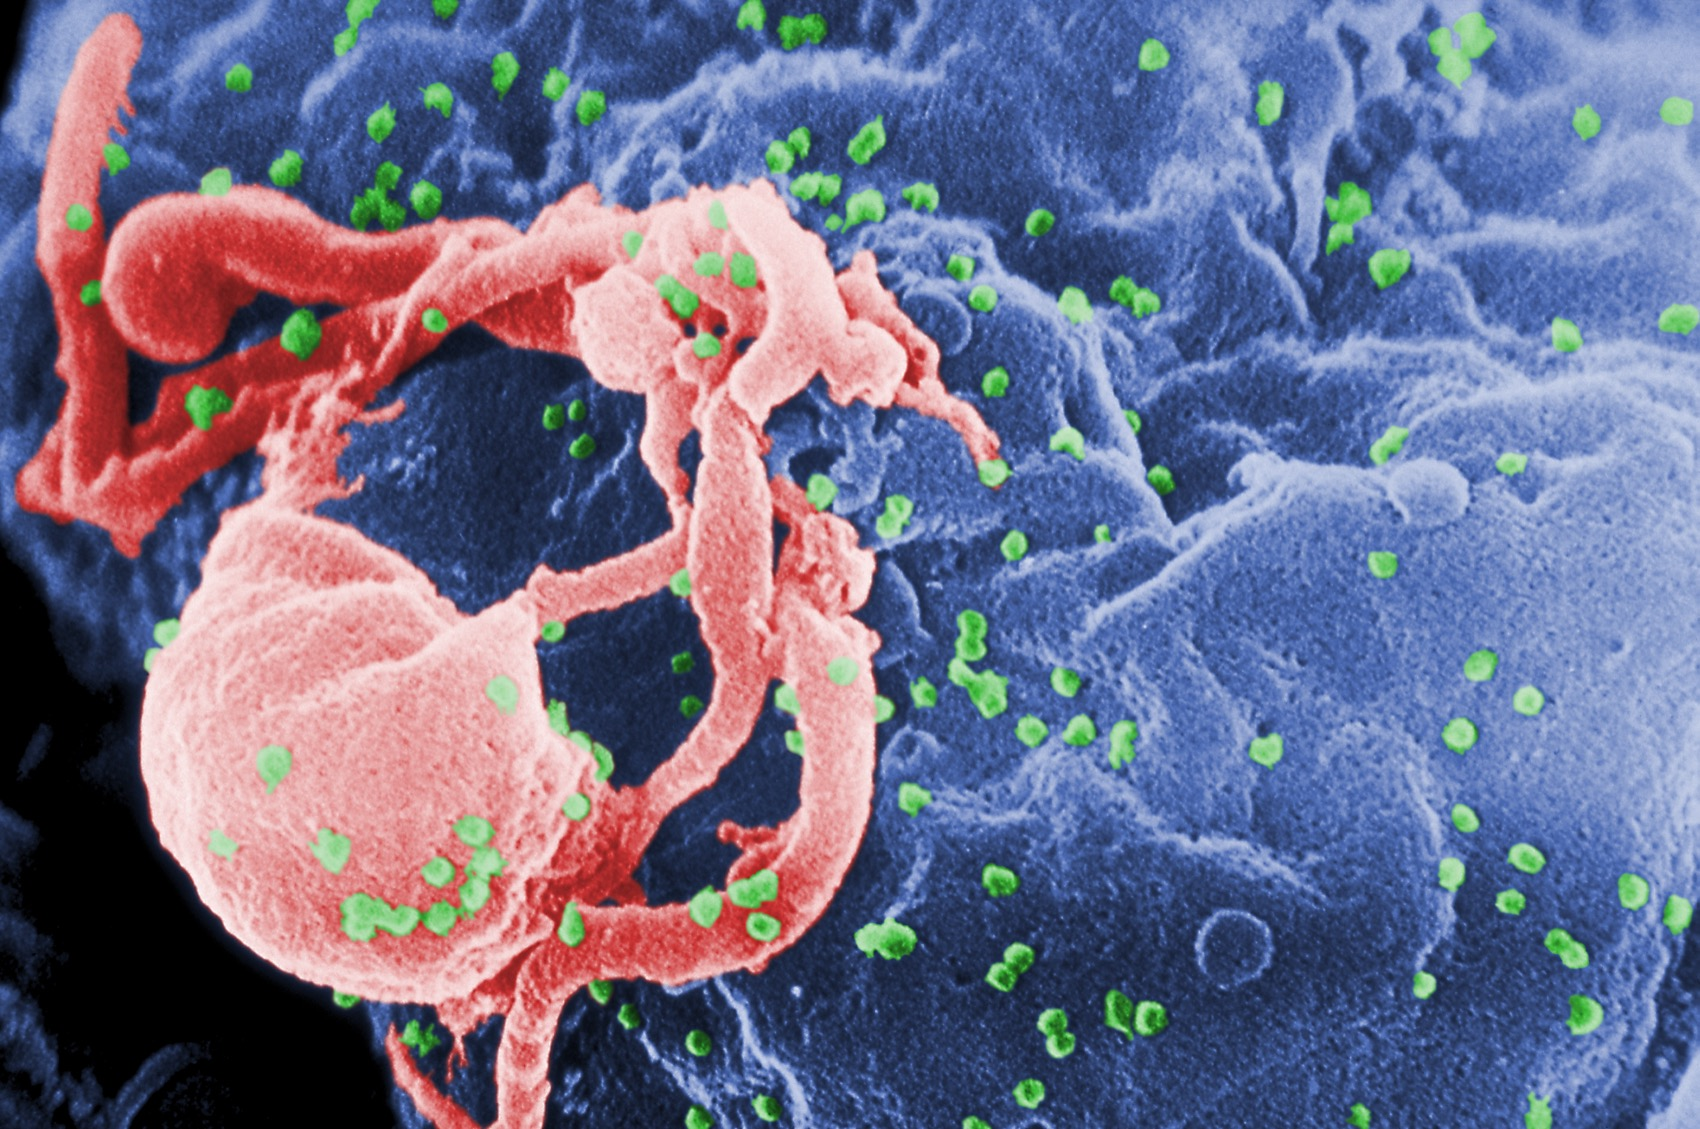
\includegraphics[width=0.72\textwidth]{figures/fig_budding/hiv_budding}
\caption{Budding release. Scanning electron micrograph of HIV-1 virions
(green) assembling and departing from the surface of a cultured lymphocyte,
each bump a separate event and the cell intact. Release and death are
independent here, which is why the standard model's two constants describe such
a cell exactly. A bursting pathogen does the opposite: nothing leaves while the
load accumulates, and then everything leaves at once, in the event that ends
the cell --- and no pair of constants describes that.
\Mextref{p:ch:one-cell-to-population}{Chapter~6} turns on the difference.
Image: CDC Public Health Image Library \#10000, photo credit C.~Goldsmith.}
\label{fig:hiv_budding}
\end{figure}

\subsubsection*{Something in between?}

The recent work on HIV release reveals that the story may not be so simple as
was previously assumed --- that in cases of non-lytic virulence there may be
various strategies we are not fully aware of. Another example of something in
between bursting and budding is release by extracellular vesicles. Among
viruses that leave the cell non-lytically, a subdivision may be made into those
which produce and assemble their own protein shell to harbour genetic material,
and those which exploit the cell membrane to produce a lipid container. Of this
second group it has been known for a while that in some cases multiple
individual viruses are contained and released in one ex-membrane capsule; these
are referred to as extracellular vesicles \cite{kerviel2021new,buzas2023roles},
and they present another potential complexity to the story of viral release.

\vspace{4pt}
\noindent
What decides whether any of this matters is not the schedule by itself. At
fixed total output per cell and a defence that removes free particles at a
constant rate, bursting and budding give exactly the same reproduction number;
the schedule becomes visible only when the defence can be used up, or when the
quantity of interest is the chance of establishment rather than a mean.
\Mextref{p:ch:one-cell-to-population}{Chapter~6} and
\mextref{path:ch:pathogenesis}{Chapter~8} make that statement precise, and find
that the comparison reverses according to whether the defence facing a release
is a rate or a finite budget.
